\chapter{State of the Art}

This chapter presents the state of the art that will set the stage for the work developed in this dissertation.

\section{E-mail and .eml}

E-mail, short for electronic mail, is a method of exchanging messages over the internet or computer networks. It is one of the most widely used forms of digital communication today, with billions of users worldwide. E-mail remains a central medium not only for legitimate communication but also as a primary attack vector exploited by cybercriminals through phishing and malware distribution.

From a technical perspective, e-mail is structured according to the Internet Message Format (\acs{RFC} 5322), which defines the standard headers and body content of a message, such as sender, recipient, subject, date, and message body \cite{rfc5322}. This specification was later updated by \acs{RFC} 6854, which introduced support for group syntax in the From: and Sender: header fields, thereby allowing messages to represent multiple authors or senders in a structured and standardized manner \cite{rfc6854}. Individual messages can be stored and exchanged as .eml files, a format that encapsulates the full message including metadata (headers), body text, and attachments using the MIME standard. The .eml format is particularly relevant in research contexts, as it preserves raw information such as authentication results, routing paths, and content features that are useful for forensic analysis and machine learning-based detection approaches.

As one of the most popular communication tools, e-mail has become a prime target for cyber attacks. Its widespread use, combined with the inherent trust users place in messages that appear legitimate, makes e-mail an ideal vector for malicious actors seeking to steal sensitive information, distribute malware, or manipulate recipients into performing certain actions. Among the various threats that exploit e-mail, phishing has emerged as one of the most prevalent and damaging, leveraging social engineering techniques to deceive users into revealing credentials, financial information, or other confidential data.

\section{Phishing}

Phishing is a type of cyber attack in which an attacker attempts to deceive individuals into providing sensitive information, such as usernames, passwords, or financial details, by disguising as a trustworthy entity through electronic communication channels, most commonly e-mail. Phishing attacks often employ social engineering tactics, exploiting users’ trust, fear, or curiosity, and can include malicious links, fraudulent websites, or deceptive attachments.

In 2024, according to the \ac{APWG}, phishing attacks have been on a decline, totaling 3.7 million attacks, down roughly 24\% from 2023.

\begin{figure}[ht]
    \centering
    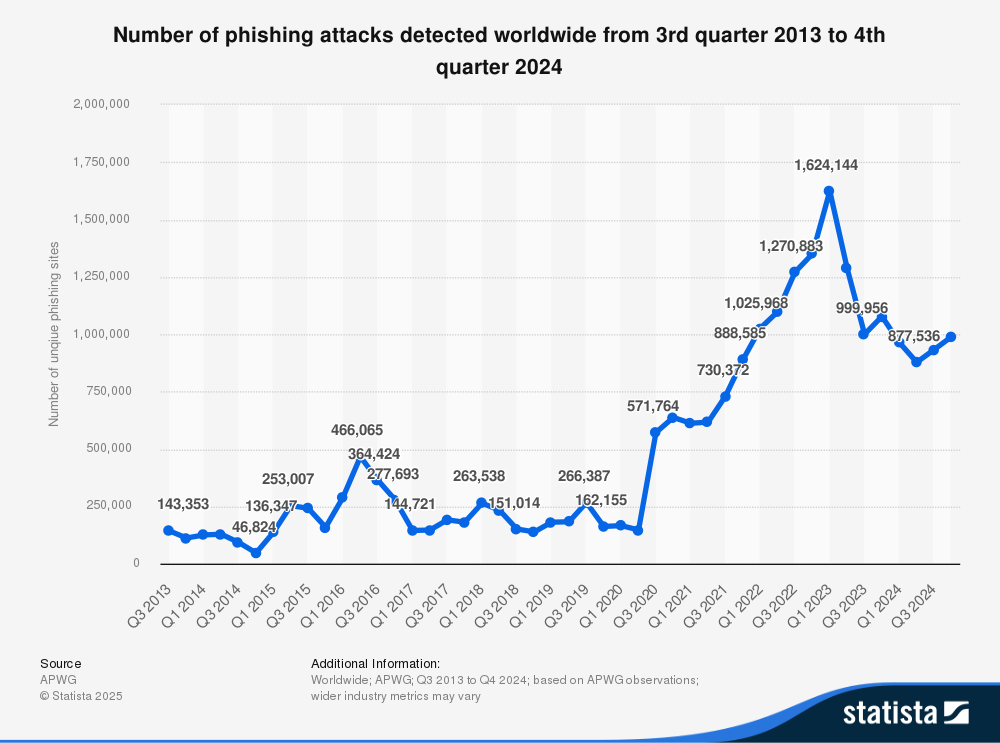
\includegraphics[width=0.8\textwidth]{figs/phishing_trends.png}
    \caption{Number of Phishing Attacks over time (Source: APWG)}
    \label{fig:phishing_trends}
\end{figure}

Although a decrease in attacks is a positive sign, phishing remains a significant threat due to its adaptability and the increasing sophistication of attacks. According to the \acs{IC3} 2024 \acs{FBI} report, phishing attacks resulted in the loss of USD 70 million, clearly showing that phishing is still a relevant threat \cite{IC32024}. These attacks often coincide with larger data breaches, further magnifying their impact on organizations and individuals.

To mitigate the threat of phishing, a wide range of technical solutions has been developed. 
These include email authentication protocols such as \ac{SPF}, \ac{DKIM}, and \ac{DMARC}, which help verify the legitimacy of senders and reduce the likelihood of spoofed messages reaching users’ inboxes \cite{DEROUET20165}.

Transport-layer protections like \ac{MTA-STS} and \ac{TLS} reporting further strengthen the security of email delivery, ensuring that messages are transmitted securely between servers and are less vulnerable to interception or tampering.

Additionally, advanced \ac{ML} and \ac{DL} approaches have been increasingly applied to detect phishing attempts. Models can leverage features extracted from email headers, body content, URLs, and attachments, with recent transformer-based architectures and embedding techniques providing state-of-the-art performance in identifying both traditional and sophisticated phishing messages.

\section{Machine Learning and Deep Learning for Phishing Detection}

\ac{ML} and \ac{DL} approaches have been the subject of extensive research in the context of phishing detection.
Attackers have been using \ac{AI} to create more convincing phishing emails, and as such, researchers are increasingly focusing on developing robust detection mechanisms that can adapt to evolving threats.

Traditional machine learning techniques are no longer sufficient to combat the sophisticated nature of modern phishing attacks \cite{Fernandes2024}. Most systems relied heavily on engineered features extracted from emails, including header fields (such as \textit{sender} or \textit{received} chain), lexical and textual cues (e.g. \ac{TF-IDF} and bag-of-words), URL tokenization, structural HTML features, and attachment metadata. These features were typically fed into classical classifiers, such as \ac{SVM}, Random Forests, Naive Bayes, or Logistic Regression. Early deep learning models, including \acp{CNN} and \acp{RNN}/\ac{LSTM}, were also applied to textual and structural components, providing promising results but still often being outperformed by well-engineered classical approaches. 

Since then, there have been several significant advances in the \ac{ML}/\ac{DL} space for email-based phishing detection:

Pretrained transformer architectures, like \ac{BERT}, \ac{DistilBERT}, and \ac{RoBERTa}, have been fine-tuned for phishing detection tasks. These models effectively encode the email body, subject lines, and sometimes HTML structure into embeddings that capture semantic and contextual signals beyond simple lexical overlaps \cite{uddin2025}.

Modern systems more often integrate multiple input modalities: authentication metadata (\ac{SPF}/\ac{DKIM}/\ac{DMARC}), header features, embedding representations of textual content, URL encoders, HTML structure features, and outputs from attachment analysis or sandbox environments \cite{PATRA2025110403, electronics12204261}.

Another technique used to detect phishing is vector similarity search. This technique involves converting raw emails into high-dimensional vectors using transformer embeddings. These vectors can then be compared to identify similarities between emails, using methods such as cosine similarity or Euclidean distance. Although this approach yielded better results than traditional \ac{ML} techniques, it was still outperformed by fine-tuned transformer models~\cite{PATRA2025110403}.

\section{Sentiment Analysis}

While most research focuses on technical and structural features of phishing emails, a section of analysis that has been largely overlooked is sentiment analysis.

Sentiment analysis involves using \ac{NLP} techniques to identify and extract subjective information from text, such as emotions, opinions, or attitudes. In the context of phishing detection, sentiment analysis can provide insights into the emotional tone and persuasive strategies employed by attackers. This can help cyber security professionals better understand the psychological tactics used, and possibly protect email users from said entity of being targeted by certain tactics, like blackmail.

In previous works, sentiment or tone was occasionally used as one auxiliary signal: existing works might include keyword frequency (urgency / fear words), lexical heuristics (e.g. counts of exclamation marks, imperative mood etc.). However, these were generally simpler, lexicon-based or manually curated features.

Most models prioritized content / URL / header / attachment features, leaving sentiment / emotional tone as a minor axis of research. This, combined with the fact that in many datasets, the emotional manipulation was implicit rather than explicitly annotated, meant that sentiment features were often noisy or under-utilized.

In a recent work, \ac{DistilBERT} was used to extract embeddings that carry sentiment / tone information, that was fed into a classical \ac{SVM}. This was compared to simply using \ac{SVM} by itself, and the results showed that the sentiment-aware model outperformed the baseline by a 3\% margin in F1-score (97\% vs 94\%) \cite{salian2024enhancing}.

Another work, "Comparative Investigation of Traditional Machine-Learning Models and Transformer Models for Phishing Email Detection", explicitly stated that results could be further improved by "incorporating sentiment analysis techniques to detect social-engineering tactics and to better understand the emotional tone and intent behind the email content" \cite{electronics13244877}.

As such, its clear that a well annotated dataset with sentiment labels, not just positive / negative labels, could provide valuable insights into the emotional manipulation tactics used in phishing emails, and potentially improve detection performance.

\section{Datasets}

A wide variety of datasets have been used in phishing detection research, ranging from legacy corpora to recently curated collections. Classic datasets such as the Enron E-mail Corpus (released in 2004 during litigation) and the SpamAssassin Public Corpus (2002) remain popular for providing large numbers of benign or spam-related messages, though their age and lack of phishing-specific samples limit their representativeness in modern studies \cite{metsis2006spam,klimt2004enron}. Similarly, the Nazario Phishing Corpus (2006) offered one of the earliest phishing-only collections, though its small size ($\approx 2,000$ messages) and outdated content restrict its usefulness today.

More recent works leverage community-driven sources such as PhishTank, which provides continuously updated phishing URLs, and the \ac{APWG} eCrime Exchange, which offers large feeds of malicious URLs and e-mails to members. These sources have been central to many detection systems but often lack full .eml message structures, making them less suitable for header or attachment-based analysis \cite{mahmoud2023phishing}.

The limitations of these datasets have driven recent efforts to curate larger, more representative corpora. For example, Champa et al. (2025) compiled seven curated phishing datasets totaling over 200,000 instances, addressing the scarcity of structured corpora for ML research \cite{champa2025curated}. Similarly, Caripoti et al. (2025) proposed E-PhishGen, a framework for generating realistic phishing emails using large language models (LLMs), designed to overcome dataset scarcity and linguistic limitations in prior corpora \cite{caripoti2025ephishgen}. Another recent initiative, the EPVME dataset (2024), introduced by Patra et al., aggregates over 600,000 malicious and benign samples while simulating novel attack vectors and vulnerabilities, offering a large-scale benchmark for modern detection techniques \cite{patra2024epvme}.

In addition, there has been increasing interest in synthetic or augmented datasets, where generative models or adversarial methods are used to produce new phishing e-mails. For instance, Caripoti (2024) created a dataset of over 10,000 phishing and legitimate samples, categorized by attack type (malware, credential harvesting, business email compromise), and showed how synthetic data could improve detection robustness across models \cite{caripoti2024synthetic}.

Together, these efforts reflect a clear evolution: while early works relied on small, static corpora, the current state of the art emphasizes large, diverse, and dynamically updated datasets. These developments also highlight the need for open, realistic .eml-based datasets that preserve the structural, textual, and metadata features of modern phishing campaigns, a gap that motivates the construction of new datasets like the one proposed in this thesis.

\begin{table}[ht]
\centering
\caption{Commonly Used Datasets in Phishing Detection Research}
\label{tab:phishing_datasets}
\begin{tabular}{|p{3cm}|p{3cm}|p{4cm}|p{5cm}|}
\hline
\textbf{Dataset / Corpus} & \textbf{Year / Source} & \textbf{Size \& Content} & \textbf{Notes / Usage in Literature} \\ \hline
Enron E-mail Corpus & Released $\sim$2004 (Enron litigation) & $\sim$500,000 corporate e-mails (benign) & Widely used for legitimate e-mail baseline; not security-focused, language is outdated. \\ \hline
SpamAssassin Public Corpus & 2002 (Apache SpamAssassin project) & $\sim$6,000 e-mails (spam + ham) & Includes spam, phishing-like, and ham; relatively small, limited diversity. \\ \hline
Nazario Phishing Corpus & $\sim$2006 (Jose Nazario collection) & $\sim$2,000 phishing e-mails & Historic phishing dataset, small and outdated but influential in early studies. \\ \hline
PhishTank & Ongoing (community-driven, OpenDNS) & URLs + associated phishing samples & Still widely used, but primarily URL-based; lacks full \texttt{.eml} structure. \\ \hline
APWG eCrime Exchange & Ongoing (Anti-Phishing Working Group) & Large, dynamic feeds of phishing URLs/e-mails & Research access restricted; provides up-to-date, real-world campaigns. \\ \hline
Custom / Proprietary Datasets & 2015--present (industry, e.g., Microsoft, Symantec) & Millions of real e-mails, often not public & Used in cutting-edge papers; limited reproducibility for academia. \\ \hline
Augmented / Synthetic Data & Recent works (2020s) & Varies (often 10k--100k+ samples) & Generated via adversarial text models or heuristics to simulate modern phishing tactics. \\ \hline
\end{tabular}
\end{table}
